\documentclass[thesis.tex]{subfiles}
\begin{document}
\chapter{Computational Optimizations [[Perhaps a more introductory title -- reserving this title for another section or chapter where is more appropriate]]}

[[I am really glad to see this section start to develop, but when you get a chance to add a bunch of meta-discourse/introduction that would be great.  Why C instead of C++ -- type of discussion. Where learn C -- ``... the hard way.''  Some overall  comments on programming and hardware for N-body simulations.  Vectors are clearly very cool, but it seems a bit deep for a start. Indicate level of computer science education that you are writing for and give your old texts are refs. For example, compiler definition.  ]]

Simulating a galaxy requires a massive amount of computational power [[OK, even a neophyte has to know that there are a huge number of stars in a galaxy.]]. Even a simple statistical approximation, with a couple hundred or thousand bodies, [[ ``statistical approximation''  meaning? You are referring to the idea of approximating, say, 100, stars by one body, no?]] involves hundreds of thousands of calculations every timestep [[a lot going on in this sentence: first the approximation of numbers of stars, secondly the nature of the calculation -- gravitation and $F = m \, a$ calculations?  I looked this point is the first in the thesis where N-body calculations are mentioned, so start more basically or possibly ref. Noah]]. Multiplied by 30 updates [[``updates'' -- a technical term define, because in the beginning that same word could be interpreted by a tyro in its generic sense]] per second (to ensure smooth graphics), we quickly become responsible for hundreds of millions of calculations every second [[nice point -- good use of ``responsible'']]. To achieve that kind of performance, we need to understand how modern computer hardware functions and how various programming languages take advantage of that [[lots of writers don't use referents, but it's fairly safe to say that referents -- especially in a thesis -- are an excellent habit.]].

\subsection{Assembly and Machine Code}

[[Perhaps a basic intro. couple of sentences laying out the hierarchy of computer programs.  Include that thorough and pedagogical definition of those two kinds of code?]]

Every computer program ever written can be expressed [[rewritten ? out]] with a small set of [[need a good modifier here to foreshadow machine code?]] commands. These [[very basic commands]] commands directly manipulate memory, adding, comparing, and copying bits around [[ at the level of the computer that is just barely above individual transistors  ]]. Different types of computer processors have different sets of commands, some more extensive than others [[some sentence close to this for that intro. sentence]]. For example, [[this example is pretty good -- althought the square root reference is a real zinger ...]] the [[always define an acronym -- as you did with RISC below]] ARM processors found in smartphones have a \emph{RISC} (reduced instruction set circuit) design, which means they can perform a minimal set of operations, and more complex operations---like the square root---are expressed in terms of that small set. Other architectures, like the x86 design found in nearly all modern laptops and desktops, are referred to as \emph{CISC} (complex instruction set circuit) designs, and can do more operations without being programmed to. This design is often faster, but is more difficult to manufacture and often more expensive. In this thesis, we will exclusively focus on the x86\_64 architecture, as found in nearly all modern desktop and laptop computers [[nice sentence -- maybe an introductory-partner sentence way up at the top.]].

The set of operations a processor [[very good stuff, but it still need a little bit of support -- even a reference to Simpson's chapter, but you might be able to do it better yourself in a couple of sentences by  paraphrasing Simpsons]] can perform is referred to as the \emph{instruction set}, and is determined entirely by the physical circuit of the processor---so an x86 processor can never be turned into an ARM processor, or vice versa. As the processor runs, instructions are provided in the form of 8-bit numbers, each one corresponding to an operation. For example, the \emph{opcode} \code{0x40} (decimal 64) tells the processor to increment a given value by one. Since the processor also needs to know what data to perform the operation on, a more complete instruction would look something like \code{0x40 6c}. This instruction increments the value stored in memory at location \texttt{6c} by one.

Early programs were written [[with combinations of instructions]] like this [[one in the paragraph above ]], as long sequences of hexadecimal numbers that could be directly interpreted by the processor [[ ``directly interpreted by the processor'' I believe that I know what that clause means, but support in for the uninitiated. ]]. However, remembering dozens of opcodes was unwieldy, and finding and fixing bugs was practically impossible [[interesting claim -- why exactly?]]. Frustrated, programmers invented human-friendly names for operations and common memory locations [[ good, but needs support  ]] and wrote a tool (called an \emph{assembler}) to automatically replace them with the appropriate number [[which appropriate number?  the one that refers to a location in RAM]]. This new programming language was called \emph{assembly} [[You can see the reader's issue the definition comes after a bunch of tough stuff.]], and greatly simplified programming. For example, our instruction from [[the]] earlier [[example of a cell phone]] would be written in assembly as something like \code{INC EAX}---still opaque, but more useful than a few hexadecimal numbers. Many programs still in use today (including Unix, the basis of Mac OS X and Linux) were originally written in an assembly language [[cool]].

\subsection{The Development of High-level Languages}

Assembly was a massive improvement over typing in raw machine code, but it remained difficult to write and maintain large codebases [[define -- seems intuitive]], especially with large teams of programmers. Simple tools like conditional (if/else) blocks and loops were error-prone [[seems as though you must have gotten this knowledge from some reference, no?  If so include it here.]], and the structure of the program mimicked the inner working of the processor more than that of the human brain [[structure of the human brain ... dangerous territory ... ]]. Various \emph{programming languages} were designed to simplify the programming process, with associated \emph{compilers} to convert source code into assembly [[seems good]]. These languages featured more natural math and now-familiar constructs like the \code{for} loop and the concept of functions [[  very familiar from MATLAB -- at least for me, define/explain ]]. The most popular and enduring of these languages was C, which underlies nearly every operating system and utility [[define pedagogically]] in use today. [[Foreshadow the fundamental differences between C and, say, Python or MATLAB]] Our example instruction from earlier, written in C, is \code{i++;}---far simpler than before, and close to the notation used in mathematics.

Of course (and this [[a well-constructed referent]] should seem familiar by this point [[  not quite understanding ... point of the thesis? ]]), C had some limitations. String [[five-word Sci. Am. definition ]] handling was an exercise in frustration, and manually handling memory meant leaks (where a piece of memory is never returned to the operating system [[ good definition  ]]) were commonplace. Accessing invalid memory was all-too-common [[surely a reference would be welcome here by someone really trying to understand the claim at a deep level]], especially among new programmers, and could lead to all kinds of insidious bugs. Higher-level languages were created to deal with these problems, providing robust, error-free constructs to simplify these tasks. The first and most well-known of these languages was C++, which started out as a collection of text replacements and code generators for C and quickly evolved into a massive, full-featured language. Others followed, many keeping the basic syntax of C but automating ever-more. In general, these languages were much easier to write than C, at a significant performance cost [[  classic claim. explain why -- harks back to the difference between complied and not-compiled languages, no? ]] ---which was offset by rapid improvements in processor technology [[at least until recently, i.e. the last couple of years.]].

\subsection{Choosing a Language}
As mentioned earlier, performance is absolutely critical for our n-body simulator. Therefore, we need to be very careful when choosing a programming language for our project. Modern \emph{Interpreted languages}---which do not compile to machine code, but are run by an \emph{interpreter} or \emph{virtual machine}---like Python or C\# have too much overhead [[ true, but explain  ]] to use [[this excellent paragraph could have been foreshadowed, thereby helping the reader.]]. Their simplicity and ease of use would be very nice to have, but they just aren't fast enough for our purposes. That leaves us with the compiled languages---C and C++ the most well known among them [[at least mention fortran, no?]].

At first, C++ would seem like an obvious choice. Features like exceptions (which greatly improve error handling) and inheritance (which makes it easier to work with complex data types) are hard to live without, and most programmers have never used a language without them. However, these features also add overhead---they function as code generators, making it easy to create a lengthy and computationally complex program without realizing it. Since we can't use most of the features that make C++ what it is for performance reasons, the choice between C and C++ is mostly cosmetic---the finished codes would look very similar, and could easily be converted into each other. Since I had more experience with C from prior project and much prefer the C syntax to that of C++, I decided to use C for this project.

\subsection{Learning C}
C has a bit of a reputation. It's seen as a fragile, temperamental language, where even the smallest change can make the difference between a crash and a successful run. Pointers---the defining language feature---can be difficult to understand at first, and are far less user-friendly than the objects and arrays most languages replace them with. But it's also a very simple language, where learning a dozen keywords and a handful of concepts lets you understand just about any C program ever written. There are countless resources online for learning C, and it isn't hard to start writing simple programs. For a [[ annotated  ]] list of useful resources, see \ref{C-resources}.


\section{Hardware-based Vectors}

Let's imagine the components of an n-body simulator. We clearly need to define some kind of data type to hold essential information about a given body---its position, its velocity (collectively referred to as its \emph{state}), its mass, and possible some kind of name or numeric ID, to allow individual bodies to be tracked. In C, we would define this \code{Body} type using a \code{struct}, or compound data type. The latter fields are simple enough---C provides datatypes for both integral and non-integral numbers, and strings are easy to create. However, defining the vectors (as needed for the position and velocity) is a little trickier. A simple definition for \code{Body} is shown in listing \ref{body-def}.

\lstinputlisting[caption={This code snippet shows the definition of the \code{Body} data type. Note that the position and velocity are of the \texttt{vec3} datatype, which is not part of the C language.\label{body-def}}]{code_snippets/body_def.c}

In the past, to write a physical simulation involving vector calculations, a programmer would have to create their own definition of a vector using a \code{struct}, like we did to define a \code{Body} (a sample definition is shown in \ref{struct-vector}). They would be responsible for coding even the most basic operations---like addition and scalar multiplication---by hand, and this code would be executed like any other, with the normal overhead of a function call. However, recent x86-64 processors (anything made by Intel in the last decade) have a single-instruction, multiple-data (SIMD) coprocessor \citep{intel-simd}, which is designed to perform a given operation on multiple numbers simultaneously.

\lstinputlisting[caption={An old-style definition of a vector\label{struct-vector}}]{code_snippets/struct-vector.c}


\subsection{SIMD}
SIMD, short for \emph{single-instruction, multiple-data}, is the simplest form of parallelism. A special piece of hardware executes the same command on more than one piece of data at a time, making it very useful for tasks like array processing or graphics rendering, where each element in the array or each pixel on the screen needs the same computations performed on it. For tasks like array processing, the SIMD optimizations are often generated by the compiler, with no programmer input necessary (other than setting the correct flags). This model---where each element is computed simultaneously---would also seem to work well for basic vector operations like addition and scalar multiplication, which are calculated on an element-by-element basis. Since the compiler cannot figure out whether a given data type is meant to represent a vector, we need to explicitly tell it. The syntax for doing so is shown in listing \ref{ext-vector}.


\begin{lstlisting}[caption={The declaration for EXT vector types. These vectors are
    not part of standard C, but are available on nearly all modern systems using the \code{clang} compiler.\label{ext-vector}}]
    //This declares a new datatype called vec3.
    //It consists of double-precision floating point numbers,
    //and is defined to be a 3-dimensional vector by the
    //__attribute__ tag.
    typedef double vec3 __attribute__((ext_vector_type(3)));
\end{lstlisting}



\subsection{Properties of Hardware-based Vectors}

Although these types are meant to serve as vectors, many useful vector operations---absolute value, the cross and dot products, and similar---are not implemented. As a general rule, any operation that returns a scalar (like the absolute value and dot product, for example), or doesn't have a scalar analogue (like the cross product, which is only defined on 3-dimensional vectors), must be implemented by the programmer. Writing the code for these operations tends to be fairly simple, and uses the standard algorithms covered in Physics 101. For example, listing \ref{software-implem} shows the code for calculating the absolute value of a vector.

\begin{lstlisting}[caption={Implementing the absolute value function in software\label{software-implem}}]
    inline double vabs (vec3 v) {
        return sqrt(v.x*v.x + v.y*v.y + v.z*v.z);
    }
\end{lstlisting}

Some operations are already predefined. Since these vectors follow the SIMD model, any operation that acts on each element individually is trivial for the compiler to handle. Therefore, all of the normal C operators are valid for vectors. Sometimes, like in the case of addition or scalar multiplication, this behavior is normal and expected, and provides a useful speed improvement over a software-based method. However, some operators make no sense under this model yet are defined anyways. For example, a vector space is not an ordered field (as we learned in linear algebra). There is no good way to order or sort vectors. And yet the \code{< >} operators are defined for vectors, behaving as shown in listing \ref{operators}. This behavior can be a little tricky, especially when an operator behaves unexpectedly.

\begin{lstlisting}[caption={Some operations aren't especially useful\label{operators}}]
    (vec3){0,5,8} > (vec3){3,4,8} == (vec3){false, true, false};
\end{lstlisting}



\subsection{Performance Advantages}

Now that we have our two ways of defining vectors, we need to compare their performance. The best way to measure the performance of various kinds of vectors is to write a simple program and time it, both with and without hardware vectors enabled. However, looking at the assembly output of the compiler can also provide valuable information, since each instruction has a similar execution time. For example, listing \ref{unopt-assembly} shows the code for a performance critical loop that calculates force, compiled with the option \code{-Ofast}---which enables maximum optimizations, but still uses the old-style vectors from earlier.

Listing \ref{opt-assembly}, on the other hand, has been compiled with vector support---using options \code{-Ofast -march=native} telling the compiler to take advantage of any and all CPU features that could be useful. It is about two-thirds as long as the fastest possible software version, which generally corresponds to a 33\% performance increase---a huge boon in code that runs tens of millions of times per second. Rows and rows of near-identical \code{add} and \code{mov} calls are replaced by a single specialized call to \code{vfmadd231sd}, a vector-based instruction that performs all those operations simultaneously.

[[Need a lot of help with these listing --> if not they go to the appendix]]


\lstinputlisting[caption={The optimized assembly for a critical loop, without SIMD vector support. Don't worry if you can't understand this---neither can I. The important thing is its relative length.\label{unopt-assembly}},language={[x64]Assembler}]
{code_snippets/Oserial.s}

\lstinputlisting[caption={The same code, with SIMD vectors\label{opt-assembly}},
                    language={[x64]Assembler}]{code_snippets/Ofast.s}

\subsection{Disadvantages}
There is a good reason SIMD support is not enabled by default. Because its instructions are not part of the \texttt{x86-64} standard, various chipset manufacturers may implement the feature differently (or not enable it at all.) The \texttt{-march=native} flag we passed to the compiler voids any guarantee that the resulting binary be able to run on any computer running the same operating system and instruction set. We could build the non-SIMD code in 32-bit mode and load the resulting binary onto a computer from the early 90s, and it would (probably) run. Trying the same with the SIMD-enabled binary may throw an error similar to the one seen in \ref{SIGILL}, especially on old or lower-end CPUs.

\begin{lstlisting}[caption={An error thrown by an unsupported instruction on OS X. Running vector code on an unsupported processor would lead to something like this.\label{SIGILL}}]
	45584 illegal hardware instruction  ./a.out
\end{lstlisting}

\section{The Tree Algorithm}

By implementing hardware-based vectors, we've sped up our force-calculating function by nearly 30\%. However, running that function still takes \emph{some} amount of time, and that will remain true no matter how much we optimize it. We can---and should---fiddle around with low-level assembly all day, but at some point that strategy faces diminishing returns. There are only so many optimizations that can be squeezed out of a piece of code, and at some point we will reach the shortest possible runtime for an algorithm. At that point, the only way to speed up our computation is to do less of it, replacing chunks of calculations with good-enough approximations that take a fraction of the time to calculate.

When trying to calculate the behavior of a body in a field, the simplest way is to calculate the force on that body from every other body that makes up that field. This strategy is easy to implement---the only relevant equations are from Physics 101. However, as the number of bodies to be considered grows, the required number of computations skyrockets, becoming untenable on even the most powerful computers. In technical terms, this algorithm is said to have a \emph{time efficiency} of O$(n^2)$, which means that, as the number of bodies doubles, the number of calculations quadruples.

We clearly need to find a way to reduce the number of calculations. Using the system in figure \ref{treecode-basic} as an example, we see that each body requires 79 calculations---a good baseline to work from. Recall from Physics 101 that, as one moves further away, the forces exerted by two identical bodies near each other converge. It follows that, if distant collections of bodies could be replaced with singular large bodies, the number of calculations could be sharply reduced without significantly impacting accuracy. Figure \ref{treecode-merged} shows an example of this, replacing a cluster of 10 distant bodies and reducing the number of calculations by about 15\%---with only one replacement.

\begin{figure}[p]
	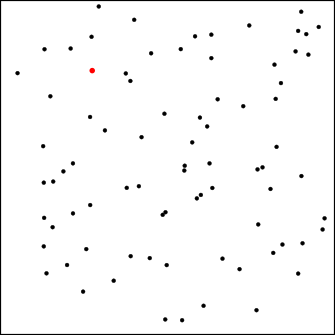
\includegraphics{imgs/treecode-basic}
	\caption{We want to calculate the force on the red dot in this system, which involves 79 calculations (since there are 80 bodies). These 79 calculations must be repeated for every other body, for a total of $79*80=6320$ calculations.}
	\label{treecode-basic}
\end{figure}

\begin{figure}[p]
	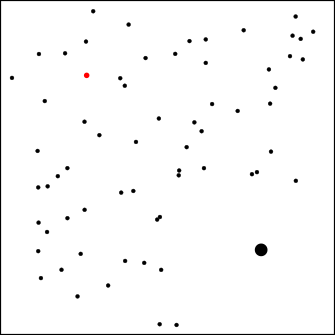
\includegraphics{imgs/treecode-merged}
	\caption{The force on the red body in this system is similar to the one seen earlier. However, the number of calculations has been significantly reduced, because about 10 bodies have been replaced with one large body.}
	\label{treecode-merged}
\end{figure}

Our next task is to find an algorithm to do all these merges and accuracy judgements as quickly as possible. Representing space as a kind of tree structure makes this easy to do. To build this tree, space is divided into nodes along each axis (so a 2-dimensional node will have 4 children, while a 3-dimensional one will have 8). Each of these child nodes is then bisected in the same manner, and the process repeats recursively until each bottom-level node has 0 or 1 bodies in it. The resulting structure is referred to as a quadtree (in 2D space) or an octotree (in 3D space). The first two levels of a quadtree can be seen in figure \ref{treecode-nodelev2}.

\begin{figure}[p]
	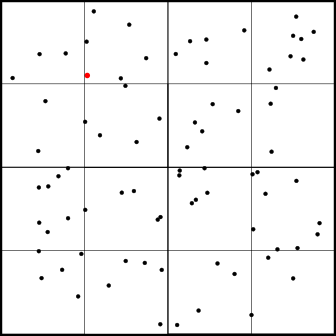
\includegraphics{imgs/treecode-nodelev2}
	\caption{The quadtree after two levels of bisections. Note the 4 child nodes of each node, and the ease of scaling this structure to an arbitrary dimension.}
	\label{treecode-nodelev2}
\end{figure}

Then, to create a system that approximates the original, we simply have to ``walk'' through the tree, deciding whether each node is a suitably accurate approximation for the bodies contained within, or whether its children should be considered individually. This decision is based on the mass of the node and its distance from the body of interest, as well as an ``accuracy factor'' that controls the allowable level of error. Eventually, a list of nodes is created that contains each body exactly once, and the net force can be found by summing up the forces from each node. Figure

\begin{figure}[p]
	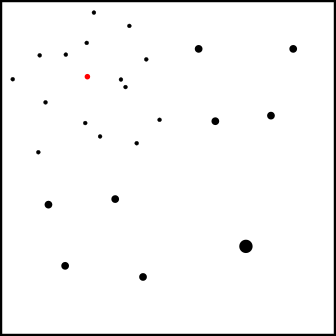
\includegraphics{imgs/treecode-nodes-final}
	\caption{This system is a good approximation of the one considered earlier, and only requires 24 calculations---nearly 75\% less than before. Of course, a real algorithm would be far more rigorous, and likely find even more opportunities to merge bodies.}
	\label{treecode-nodes-final}
\end{figure}

The algorithm discussed here has a time complexity of O$(n \log n)$ in the average case, and O$(n^2)$ in the very worst case. This means that it will practically always beat the na\"ive algorithm for systems of more than a few bodies, and becomes very valuable for large simulations. The creation and analysis of the tree does add some overhead, but a well written implementation will rarely take longer than a few dozen force calculations---while eliminating hundreds or even thousands.

\end{document}
